%\let\negmedspace\undefined
\let\negthickspace\undefined
\documentclass[journal,12pt,twocolumn]{IEEEtran}
\usepackage{gensymb}
\usepackage{amssymb}
\usepackage[cmex10]{amsmath}
\usepackage{amsmath}
\usepackage{amsthm}
\usepackage[export]{adjustbox}
\usepackage{bm}
\usepackage{longtable}
\usepackage{enumitem}
\usepackage{mathtools}
 \usepackage{tikz}
\usepackage[breaklinks=true]{hyperref}
\usepackage{listings}
\usepackage{color}                                            %%
\usepackage{array}                                            %%
\usepackage{longtable}                                        %%
\usepackage{calc}                                             %%
\usepackage{multirow}                                         %%
\usepackage{hhline}                                           %%
\usepackage{ifthen}                                           %%
\usepackage{lscape}     
\usepackage{multicol}
\usepackage{float}
% \usepackage{enumerate}
\DeclareMathOperator*{\Res}{Res}
\renewcommand\thesection{\arabic{section}}
\renewcommand\thesubsection{\thesection.\arabic{subsection}}
\renewcommand\thesubsubsection{\thesubsection.\arabic{subsubsection}}
\renewcommand\thesectiondis{\arabic{section}}
\renewcommand\thesubsectiondis{\thesectiondis.\arabic{subsection}}
\renewcommand\thesubsubsectiondis{\thesubsectiondis.\arabic{subsubsection}}
\hyphenation{op-tical net-works semi-conduc-tor}
\def\inputGnumericTable{}                                 %%
\lstset{
frame=single, 
breaklines=true,
columns=fullflexible
}
\begin{document}
\newtheorem{theorem}{Theorem}[section]
\newtheorem{problem}{Problem}
\newtheorem{proposition}{Proposition}[section]
\newtheorem{lemma}{Lemma}[section]
\newtheorem{corollary}[theorem]{Corollary}
\newtheorem{example}{Example}[section]
\newtheorem{definition}[problem]{Definition}
\newcommand{\BEQA}{\begin{eqnarray}}
\newcommand{\EEQA}{\end{eqnarray}}
\newcommand{\define}{\stackrel{\triangle}{=}}
\newcommand*\circled[1]{\tikz[baseline=(char.base)]{
    \node[shape=circle,draw,inner sep=2pt] (char) {#1};}}
\bibliographystyle{IEEEtran}
\providecommand{\mbf}{\mathbf}
\providecommand{\pr}[1]{\ensuremath{\Pr\left(#1\right)}}
\providecommand{\qfunc}[1]{\ensuremath{Q\left(#1\right)}}
\providecommand{\sbrak}[1]{\ensuremath{{}\left[#1\right]}}
\providecommand{\lsbrak}[1]{\ensuremath{{}\left[#1\right.}}
\providecommand{\rsbrak}[1]{\ensuremath{{}\left.#1\right]}}
\providecommand{\brak}[1]{\ensuremath{\left(#1\right)}}
\providecommand{\lbrak}[1]{\ensuremath{\left(#1\right.}}
\providecommand{\rbrak}[1]{\ensuremath{\left.#1\right)}}
\providecommand{\cbrak}[1]{\ensuremath{\left\{#1\right\}}}
\providecommand{\lcbrak}[1]{\ensuremath{\left\{#1\right.}}
\providecommand{\rcbrak}[1]{\ensuremath{\left.#1\right\}}}
\theoremstyle{remark}
\newtheorem{rem}{Remark}
\newcommand{\sgn}{\mathop{\mathrm{sgn}}}
\providecommand{\abs}[1]{\left\vert#1\right\vert}
\providecommand{\res}[1]{\Res\displaylimits_{#1}} 
\providecommand{\norm}[1]{\left\lVert#1\right\rVert}
%\providecommand{\norm}[1]{\lVert#1\rVert}
\providecommand{\mtx}[1]{\mathbf{#1}}
\providecommand{\mean}[1]{E\left[ #1 \right]}
\providecommand{\fourier}{\overset{\mathcal{F}}{ \rightleftharpoons}}
%\providecommand{\hilbert}{\overset{\mathcal{H}}{ \rightleftharpoons}}
\providecommand{\system}{\overset{\mathcal{H}}{ \longleftrightarrow}}
	%\newcommand{\solution}[2]{\textbf{Solution:}{#1}}
\newcommand{\solution}{\noindent \textbf{Solution: }}
\newcommand{\cosec}{\,\text{cosec}\,}
\providecommand{\dec}[2]{\ensuremath{\overset{#1}{\underset{#2}{\gtrless}}}}
\newcommand{\myvec}[1]{\ensuremath{\begin{pmatrix}#1\end{pmatrix}}}
\newcommand{\mydet}[1]{\ensuremath{\begin{vmatrix}#1\end{vmatrix}}}
\newcommand*{\permcomb}[4][0mu]{{{}^{#3}\mkern#1#2_{#4}}}
\newcommand*{\perm}[1][-3mu]{\permcomb[#1]{P}}
\newcommand*{\comb}[1][-1mu]{\permcomb[#1]{C}}
\numberwithin{equation}{subsection}
\makeatletter
\@addtoreset{figure}{problem}
\makeatother
\let\StandardTheFigure\thefigure
\let\vec\mathbf
\renewcommand{\thefigure}{\theproblem}
\def\putbox#1#2#3{\makebox[0in][l]{\makebox[#1][l]{}\raisebox{\baselineskip}[0in][0in]{\raisebox{#2}[0in][0in]{#3}}}}
     \def\rightbox#1{\makebox[0in][r]{#1}}
     \def\centbox#1{\makebox[0in]{#1}}
     \def\topbox#1{\raisebox{-\baselineskip}[0in][0in]{#1}}
     \def\midbox#1{\raisebox{-0.5\baselineskip}[0in][0in]{#1}}
\vspace{3cm}
\title{ASSIGNMENT}
\author{BT21BTECH11005 \ MANIKANTA}
% make the title area
\maketitle
\newpage
\tableofcontents
\bigskip
\renewcommand{\thefigure}{\theenumi}
\renewcommand{\thetable}{\theenumi}
\renewcommand{\theequation}{\theenumi}
\section{Uniform Random Numbers}
Let $U$ be a uniform  random variable between 0 and 1
\begin{enumerate}[label=\thesection.\arabic*.,ref=\thesection.\theenumi]
\numberwithin{equation}{enumi}
\numberwithin{figure}{enumi}
\numberwithin{table}{enumi}
\item Generate $10^6$ samples of $U$ using a C program and save into a file called uni.dat .\\
\solution Download the file:
\begin{lstlisting}
$ wget https://github.com/Manikanta0705/Assignment/blob/main/code/1-1.c
$ wget https://github.com/Manikanta0705/Assignment/blob/main/code/source.h
\end{lstlisting}
and compile and execute the C program using
\begin{lstlisting}
$ gcc 1-1.c -lm -wall -g
$ ./a.out
\end{lstlisting}
\item Load the uni.dat file into python and plot the empirical CDF of $U$ using the samples in uni.dat. The CDF is defined as\\
\solution  The following code plots Fig. \ref{fig:uni_cdf}
\begin{lstlisting}
$ wget https://github.com/Manikanta0705/Assignment/blob/main/codes/1-2.py
\end{lstlisting}
It is executed with
\begin{lstlisting}
$ python3 1-2.py
\end{lstlisting}
\begin{equation}
         F_U(x) = Pr(U \leq x)
\end{equation}
    Graph of CDF is as follow:
    \begin{figure}[H]
        \centering
  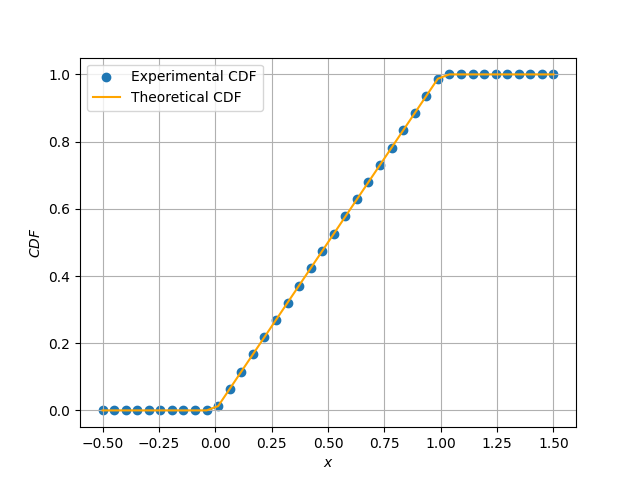
\includegraphics[scale = 0.6]{../Assignment-probability/figures/1-2.png} \label{fig:uni_cdf}
        \caption{CDF of U}
        \end{figure}
\item Find a theoretical expression for $F_U(x)$.\\
\solution Since We have,
    
    \begin{align}
    P_U(x) =  \begin{cases}
        1 & x \in (0,1) \\
        0 & otherwise
    \end{cases} 
    \end{align}
    on integrating for CDF we get,
   \begin{equation}
    F_U(x) = \int_{-\infty}^{x}P_U(t)dt
   \end{equation} 
   \begin{align}
    F_U(x) =  \begin{cases}
        \int_{-\infty}^{x}0 dx   & x \in (-\infty,0)\\
        %\int_{-\infty}^0 0 dx + 
        \int_{0}^x 1dx & x \in (0,1) \\
        %\int_{-\infty}^0 0 dx +
         \int_{0}^1 1dx & x \in (1,\infty)
 %+ \int_{1}^{x} 0 dx  & x \in (1,\infty)
    \end{cases} 
    \end{align}
    \begin{align}
    F_U(x) =  \begin{cases}
        0 & x \in (-\infty,0)\\
        x & x \in (0,1) \\
        1 & x \in (1,\infty)
    \end{cases} 
    \end{align}
\item Write a C program to find the mean and variance of U.\\
\solution download C program
\begin{lstlisting}
$ wget https://github.com/Manikanta0705/Assignment/blob/main/code/1-4.c
        \end{lstlisting}
        and compiled and executed with
        \begin{lstlisting}
$ gcc 1-4.c -lm -Wall -g
$ ./a.out
        \end{lstlisting}
    \begin{align}
        E[U] &= 0.500007  \label{eq:1.4.1}\\
        \text{Var}[U] &= 0.083301 \label{eq:1.4.2}
    \end{align}
\item Verify your result theoretically given that 
    \begin{equation}
        E[U^k] = \int_{- \infty}^{\infty} x^k dF_U(x)
    \end{equation}
    \solution we have 
    \begin{align}
        E[U] &= \int_{-\infty}^{\infty} xdF_U(x) \\
        &= \int_{0}^1 x dx \\
        &=  0.5
    \end{align}
    From \eqref{eq:1.4.1}, we have, 
    \begin{equation}
        E[U] = 0.500007 \approx 0.5
    \end{equation}
    Similarly,
    \begin{align}
        \text{Var}[U]&=E[U^2]-(E[U])^2 \\
        &=\int_{-\infty}^{\infty}x^2dF_U(x) - 0.25\\
        &=\int_{0}^{1}x^2dx - 0.25\\
        &=0.3333...-0.25=0.083333...
    \end{align}
    From \eqref{eq:1.4.2},we get
    \begin{equation}
        \text{Var}[U] = 0.083301 \approx 0.08333..
    \end{equation}
    Hence Verified.
\end{enumerate}
\section{Central Limit Theorem}
\begin{enumerate}[label=\thesection.\arabic*.,ref=\thesection.\theenumi]
\numberwithin{equation}{enumi}
\numberwithin{figure}{enumi}
\numberwithin{table}{enumi}
\item Generate $10^6$ samples of the random variable
    \begin{equation}
        X=\sum_{i=1}^{12} U_i-6        
    \end{equation}
    using a C program, where $U_i, i = 1, 2,\ldots, 12$ are a set of independent uniform random variables between 0 and 1 and save in a file called gau.dat.\\
    
    
    \solution Download the file
    \begin{lstlisting}    
$ wget https://github.com/Manikanta0705/Assignment/blob/main/code/2-1.c
    \end{lstlisting}
    Use source.h from the prob1.1\\
    And run the code as:
    \begin{lstlisting}
$ gcc 2-1.c -lm -Wall -g
$ ./a.out
\end{lstlisting}
    \item Load gau.dat in python and plot the empirical CDF of $X$ using the samples in gau.dat.
          \begin{figure}[H]
              \centering
          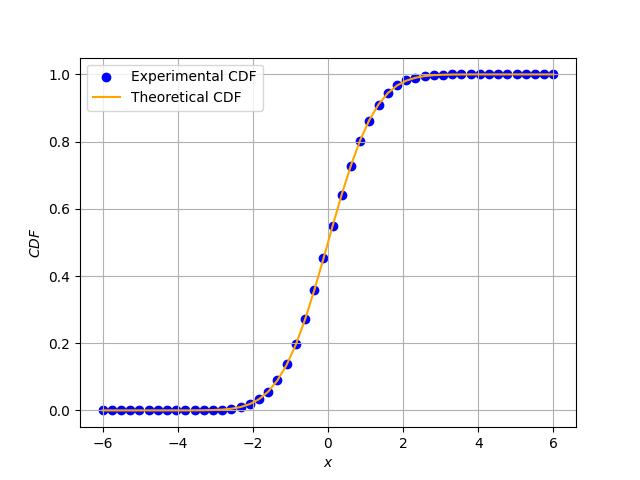
\includegraphics[width = \columnwidth]{../Assignment-probability/figures/2-2.png}
              \caption{The CDF of $X$}
              \label{fig:2-2.png}
          \end{figure}
          \solution The following gitlink plots Figure 2.2.1
          \begin{lstlisting}
wget https://github.com/Manikanta0705/Assignment/blob/main/code/2-2.py
            \end{lstlisting}
    \item Load gau.dat in python and plot the empirical PDF of $X$ using the samples in gau.dat.
          The PDF of $X$ is defined as:
          \begin{align}
              p_{X}(x) = \dfrac{d}{dx}F_{X}(x)
          \end{align}
          \begin{figure}[H]
              \centering
           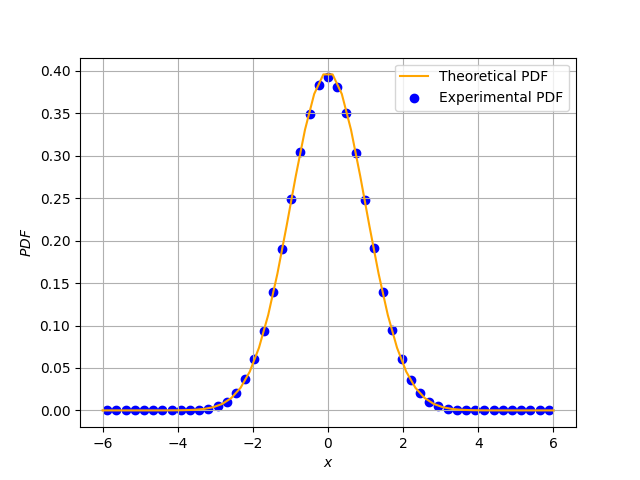
\includegraphics[width = \columnwidth]{../Assignment-probability/figures/2-3.png}
              \caption{The PDF of $X$}
              \label{fig:2-3.png}
          \end{figure}
         \solution The following git link plots Figure 2.3.1
          \begin{lstlisting}
wget https://github.com/Manikanta0705/Assignment/blob/main/code/2-3.py
            \end{lstlisting}
    \item Find the mean and variance of $X$ by writing a C program.
          \\
        \solution Download the following file:
          \begin{lstlisting}
wget https://github.com/Manikanta0705/Assignment/blob/main/code/2-4.c
            \end{lstlisting}
            and compile and execute the C program using
\begin{lstlisting}
$ gcc 2-4.c -lm -wall -g
$ ./a.out
\end{lstlisting}
          Values Obtained:
          \begin{align}
               & \fbox{Mean =  -0.000241}
               & \fbox{Variance = 1.000726}
          \end{align}
    \item Given that:
          \begin{align}
              p_{X}(x) = \dfrac{1}{\sqrt{2\pi}}\exp\brak{-\dfrac{x^2}{2}}, -\infty < x < \infty,
          \end{align}
          repeat the above exercise theoretically
          \\
          \solution
          \begin{align}
              E[X] & =  \int_{-\infty}^{\infty} \dfrac{x}{\sqrt{2\pi}}\exp{\left(-\dfrac{x^2}{2}\right)}
              \\
                   & = -\dfrac{1}{\sqrt{2\pi}}\exp\brak{-\dfrac{x^2}{2}} \Bigg{|}_{-\infty}^{\infty}
              \\
                   & = 0
          \end{align}
          Also,
          \begin{align}
              E[X^2] & =  \int_{-\infty}^{\infty} \dfrac{x^2}{\sqrt{2\pi}}\exp{\left(-\dfrac{x^2}{2}\right)}
              \\
                     & = -\dfrac{x}{\sqrt{2\pi}}e^{-\dfrac{x^2}{2}} \Bigg{|}_{-\infty}^{\infty} + \int_{-\infty}^{\infty} \dfrac{1}{\sqrt{2\pi}}e^{-\dfrac{x^2}{2}}
              \\
                     & = 0 + \dfrac{1}{\sqrt{2\pi}} \times \sqrt{2\pi}
              \\
                     & = 1
          \end{align}
          Thus,
          \begin{align}
              \text{var}(X) & = E[X^2] - E[X]^2 \\
                            & = 1
          \end{align}
          Therefore, the mean is $0$ and the variance is $1$.
          \begin{align}
              \pr{X > x} & = Q\brak{Z > x}
              \\
                         & = Q\brak{z}
              \\
              CDF        & = \pr{X < x}
              \\
                         & = 1 - Q\brak{z}
          \end{align}
\end{enumerate}
\section{From Uniform to Other}
\begin{enumerate}[label=\thesection.\arabic*,ref=\thesection.\theenumi]
    \item
          Generate samples of:
          \begin{equation}
              V = -2\ln\brak{1-U}
          \end{equation}
          and plot its CDF.
          \\
          \solution
          \begin{figure}[H]
              \centering
              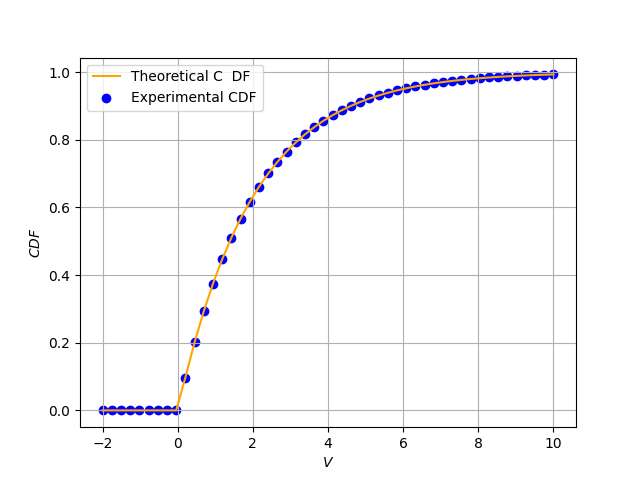
\includegraphics[width = \columnwidth]{../Assignment-probability/figures/3-1.png}
              \caption{The CDF of $V$}
              \label{fig:3_cdf}
          \end{figure}
        The following  plots Figure 3.1.1
          \begin{lstlisting}
wget https://github.com/Manikanta0705/Assignment/blob/main/codes/3-1.py
            \end{lstlisting}
    \item Find a theoretical expression for $F_V(x)$.
          \\
          \solution
          \begin{align}
              F_V(x) & = \pr{V \leq x}
              \\
                     & = \pr{-2\ln(1-U) \leq x}
              \\
                     & = \pr{1-U \geq	\exp{\left(-\dfrac{x}{2}\right)}}
              \\
                     & = \pr{U \leq 1 - \exp{\left(-\dfrac{x}{2}\right)}}
              \\
                     & = F_U\left(1 - \exp{\left(-\dfrac{x}{2}\right)}\right)
          \end{align}
          Therefore,
          \begin{align}
                       & F_V(x) =
              \begin{cases}
                  0,                                    & 1 - \exp{\left(-\dfrac{x}{2}\right)} \in (-\infty,0)
                  \\
                  1 - \exp{\left(-\dfrac{x}{2}\right)}, & 1 - \exp{\left(-\dfrac{x}{2}\right)} \in (0,1)
                  \\
                  1,                                    & 1 - \exp{\left(-\dfrac{x}{2}\right)} \in (1, \infty)
              \end{cases}
              \\
              \implies & F_V(x) =
              \begin{cases}
                  0,                                    & x \in (-\infty,0)
                  \\
                  1 - \exp{\left(-\dfrac{x}{2}\right)}, & x \in (0,\infty)
              \end{cases}
          \end{align}
\end{enumerate}

\end{document}

        
 